\documentclass[10pt]{article}
\usepackage[a4paper,margin=1.8cm,headheight=16pt,headsep=10pt]{geometry}
\usepackage{fontspec}
\usepackage[table,dvipsnames]{xcolor}
\usepackage{tikz}
\usetikzlibrary{positioning,arrows.meta,fit,backgrounds,calc}
\usepackage{booktabs}
\usepackage{array}
\usepackage{longtable}
\usepackage{enumitem}
\usepackage{fancyhdr}
\usepackage{graphicx}
\usepackage[hidelinks]{hyperref}

% ── Paleta Clinical Indigo ───────────────────────────────────────────────────
\definecolor{indigo}{HTML}{1A237E}
\definecolor{accent}{HTML}{3D6FD6}
\definecolor{ink}{HTML}{1A1F2B}
\definecolor{soft}{HTML}{55607A}
\definecolor{codebg}{HTML}{F4F6FB}
\definecolor{panelb}{HTML}{EEF2FB}
\definecolor{engine}{HTML}{E3ECFF}
\definecolor{rulec}{HTML}{C9D2E6}
\definecolor{warnbg}{HTML}{FFF7EA}
\definecolor{warnbd}{HTML}{D79A12}
\definecolor{rowalt}{HTML}{F6F8FC}

% ── Fuentes del sistema ──────────────────────────────────────────────────────
\setmainfont{Helvetica Neue}
\newfontfamily\hf{Avenir Next}
\setmonofont[Scale=0.82]{Menlo}

\setlength{\parindent}{0pt}
\setlength{\parskip}{4pt}
\renewcommand{\arraystretch}{1.28}

% ── Encabezado / pie ─────────────────────────────────────────────────────────
\pagestyle{fancy}\fancyhf{}
\fancyhead[L]{\footnotesize\hf\color{soft}EpiForecast-MX\;\textbullet\;Guía de Entrega de Patente}
\fancyhead[R]{\footnotesize\hf\color{soft}Patent Delivery Guide}
\fancyfoot[C]{\footnotesize\color{soft}\thepage}
\renewcommand{\headrule}{\vskip2pt{\color{rulec}\hrule height 0.6pt}}
\renewcommand{\footrulewidth}{0pt}

% ── Helpers ──────────────────────────────────────────────────────────────────
\newcommand{\msec}[2]{\vspace{8pt}\par
  {\hf\bfseries\large\color{indigo}#1\ \ \textcolor{accent}{\textbar}\ \ {\itshape\mdseries\color{soft}#2}}\par
  \vspace{1pt}{\color{accent}\hrule height 1.3pt}\vspace{5pt}}
\newcommand{\noticebox}[1]{\par\begin{tikzpicture}\node[fill=warnbg,draw=warnbd,line width=1pt,
  rounded corners=4pt,inner sep=10pt,text width=\dimexpr\linewidth-24pt\relax]{#1};\end{tikzpicture}\par}
\newcommand{\codebox}[1]{\par\colorbox{codebg}{\parbox{\dimexpr\linewidth-2\fboxsep\relax}{\ttfamily\small #1}}\par}
\newcommand{\es}[1]{{\small\textbf{\color{indigo}ES\ \ }#1}\par}
\newcommand{\en}[1]{{\small\textbf{\color{accent}EN\ \ }\itshape#1}\par}

\begin{document}

% ── Portada ──────────────────────────────────────────────────────────────────
\begin{center}
{\hf\bfseries\fontsize{26}{30}\selectfont\color{indigo}EpiForecast-MX}\\[3pt]
{\hf\Large\color{ink}Guía de Entrega de Patente\ \ \textcolor{accent}{\textbar}\ \ Patent Delivery Guide}\\[7pt]
{\color{soft}Árbol curado del código de la invención\ \textbullet\ Curated invention code bundle}\\[2pt]
{\color{soft}\footnotesize Generado por \texttt{scripts/build\_patent\_bundle.sh}\ \textbullet\ $\sim$262 archivos / 2.4 MB\ \textbullet\ \texttt{IntegradorIMSS2026Team01/EpiForecast-MX-Patente}}
\end{center}
\vspace{-2pt}{\color{accent}\hrule height 2pt}
\vspace{6pt}

% ── 1. Resumen ───────────────────────────────────────────────────────────────
\msec{Resumen}{Overview}
\es{Este paquete contiene \textbf{únicamente la invención} y la evidencia de que funciona: el código de los motores, su configuración, la orquestación y las pruebas. Se excluye todo el material documental voluminoso, los datos clínicos del IMSS y los binarios de modelos. El repositorio completo pesa $\sim$5.5\,GB; la invención son $\sim$2.4\,MB.}
\en{This bundle ships \textbf{only the invention} and the evidence that it works: the engine code, its configuration, the orchestration and the tests. All documentary bloat, the clinical IMSS data and the model binaries are excluded. The full repository is $\sim$5.5\,GB; the invention is $\sim$2.4\,MB.}

% ── 2. Estructura: carpeta y componente ──────────────────────────────────────
\msec{Estructura: carpeta y componente}{Structure: folder and component}
{\renewcommand{\arraystretch}{1.08}\setlength{\tabcolsep}{4.5pt}\small
\rowcolors{2}{rowalt}{white}
\begin{longtable}{>{\raggedright\arraybackslash}p{2.95cm} >{\raggedright\arraybackslash}p{3.3cm} >{\raggedright\arraybackslash}p{9.7cm}}
\rowcolor{indigo}
{\color{white}\hf\bfseries Carpeta / Folder} & {\color{white}\hf\bfseries Componente / Component} & {\color{white}\hf\bfseries Rol / Role}\\
\endhead
\texttt{src/epiforecast/} & Paquete principal \textbar\ Core package & La invención: $\sim$15k LOC. \textit{The invention.}\\
\quad\texttt{models/} & 5 motores + Factory & Prophet, DeepAR, Ensemble, Stacking, NBGLM; \texttt{factory.py}, \texttt{base.py} ($@$\,register\_model). \textit{Five engines + Factory/Strategy.}\\
\quad\texttt{data/} & Ingesta y preprocesamiento & Extracción de PDFs SINAVE, regresor ENSO/ONI, limpieza y transformación. \textit{SINAVE PDF extraction, ENSO regressor, preprocessing.}\\
\quad\texttt{features/} & Ingeniería de variables & Variables demográficas y de calendario. \textit{Demographic and calendar features.}\\
\quad\texttt{evaluation/} & Métricas & RMSE, MAE, MAPE, SMAPE, MASE. \textit{Forecast metrics.}\\
\quad\texttt{visualization/} & Gráficas y reportes & Figuras y reportes HTML estilo institucional. \textit{Charts and HTML reports.}\\
\quad\texttt{utils/} & Configuración y ayudantes & Carga OmegaConf, cohortes, rutas. \textit{Config loading, cohorts, paths.}\\
\quad\texttt{pipelines/} & Pipeline base & Esqueleto de orquestación. \textit{Base pipeline skeleton.}\\
\texttt{scripts/} & Orquestación CLI & \texttt{entrena}, \texttt{predice}, \texttt{reselect\_motor\_2026}, \texttt{produccion\_dengue}, \texttt{pronostico\_congelado}, \texttt{build\_patent\_bundle}. \textit{CLI entry points.}\\
\texttt{config/} & Configuración YAML & Modelo activo, hiperparámetros, preprocesamiento (OmegaConf). \textit{Active model, hyperparameters (config-driven method).}\\
\texttt{epi\_modules/} & Consola interactiva EPI & TUI de operación (periférico). \textit{Interactive operator console (peripheral).}\\
\texttt{tests/} & Pruebas & $\sim$915 pruebas en 56 archivos. \textit{$\sim$915 tests, evidence of correctness.}\\
\texttt{docs/} & Documentación técnica & Model cards + informe de arquitectura. \textit{Model cards + architecture report.}\\
\texttt{pyproject.toml}\newline\texttt{requirements.txt}\newline\texttt{Makefile} & Build y dependencias & Paquete \texttt{epiforecast} (flit), deps fijadas, orquestación. \textit{Buildable from a clean clone.}\\
\end{longtable}}

\newpage
% ── 4. Arquitectura ──────────────────────────────────────────────────────────
\msec{Arquitectura}{Architecture}
\begin{center}
\resizebox{\linewidth}{!}{%
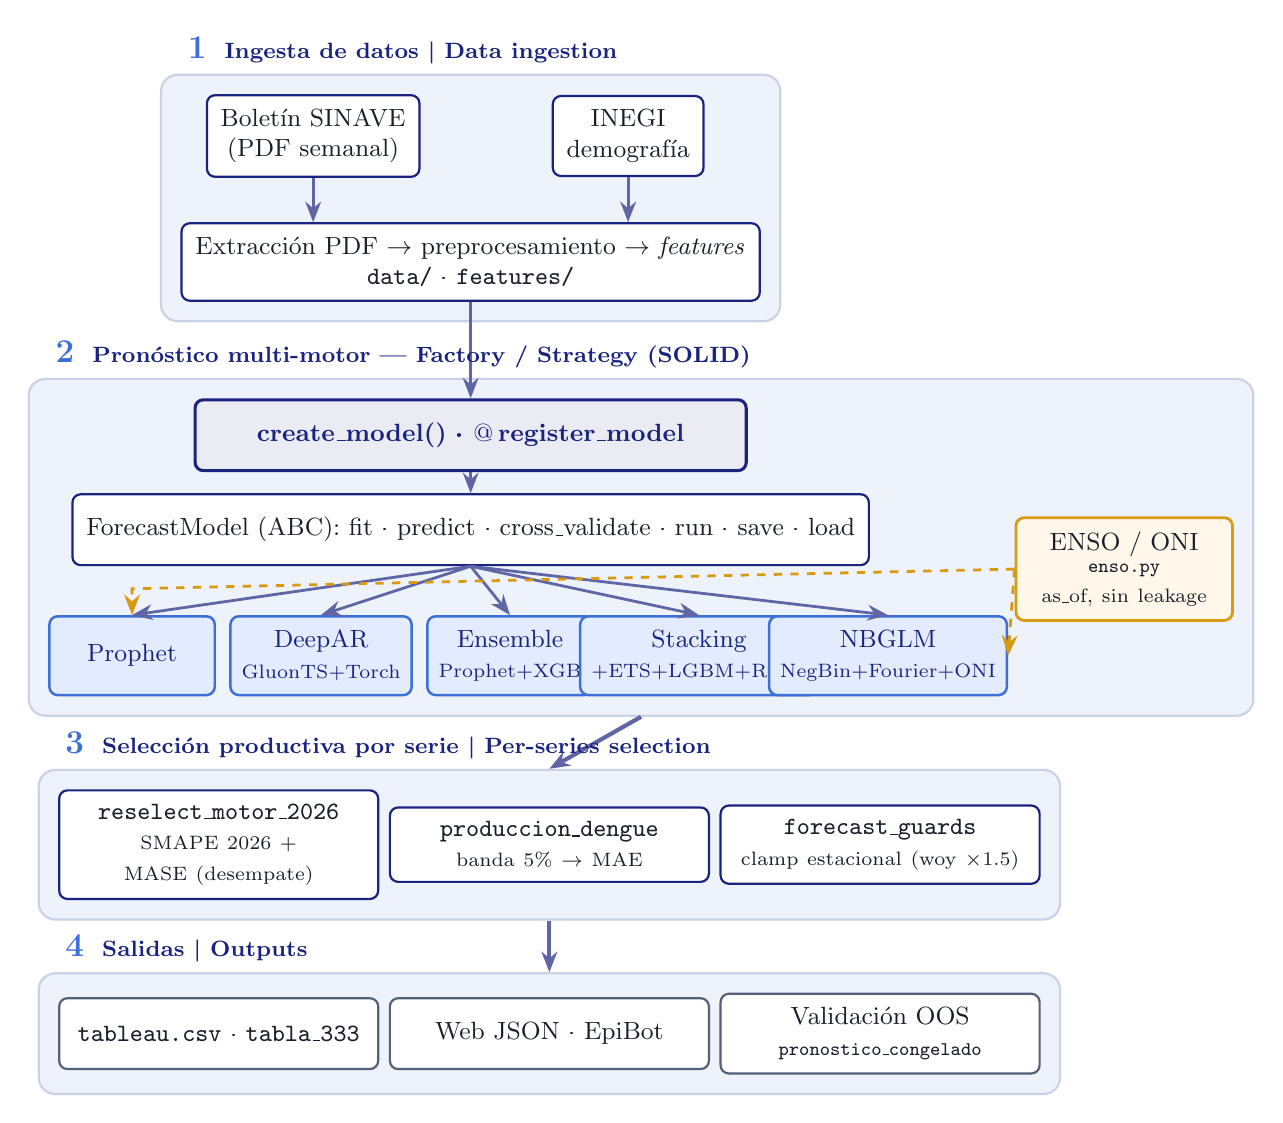
\begin{tikzpicture}[
  proc/.style={rectangle, rounded corners=3pt, draw=indigo, line width=0.8pt, fill=white, inner sep=5pt, align=center, font=\small, text=ink, minimum height=9mm},
  eng/.style={rectangle, rounded corners=3pt, draw=accent, line width=0.9pt, fill=engine, inner sep=4pt, align=center, font=\small, text=indigo, minimum height=10mm, minimum width=21mm},
  core/.style={rectangle, rounded corners=3pt, draw=indigo, line width=1.1pt, fill=indigo!9, inner sep=5pt, align=center, font=\small\bfseries, text=indigo, minimum height=9mm},
  enso/.style={rectangle, rounded corners=3pt, draw=warnbd, line width=1pt, fill=warnbg, inner sep=5pt, align=center, font=\small, text=ink, minimum height=9mm},
  outb/.style={rectangle, rounded corners=3pt, draw=soft, line width=0.8pt, fill=white, inner sep=5pt, align=center, font=\small, text=ink, minimum height=9mm},
  flow/.style={-{Stealth[length=2.6mm,width=2mm]}, draw=indigo!70, line width=1pt},
  climflow/.style={-{Stealth[length=2.6mm,width=2mm]}, draw=warnbd, line width=1pt, dashed},
  plabel/.style={font=\footnotesize\bfseries\hf, text=indigo, anchor=south west},
]
% Stage 1
\node[proc] (pdf) at (1.6,16.2) {Boletín SINAVE\\(PDF semanal)};
\node[proc] (inegi) at (5.6,16.2) {INEGI\\demografía};
\node[proc, minimum width=70mm] (prep) at (3.6,14.6) {Extracción PDF $\rightarrow$ preprocesamiento $\rightarrow$ \emph{features}\\\texttt{data/}\ \textperiodcentered\ \texttt{features/}};
\draw[flow] (pdf) -- (prep.north -| pdf);
\draw[flow] (inegi) -- (prep.north -| inegi);
% Stage 2
\node[core, minimum width=70mm] (fac) at (3.6,12.4) {create\_model() \textperiodcentered\ $@$\,register\_model};
\node[proc, minimum width=70mm] (base) at (3.6,11.2) {ForecastModel (ABC): fit \textperiodcentered\ predict \textperiodcentered\ cross\_validate \textperiodcentered\ run \textperiodcentered\ save \textperiodcentered\ load};
\node[eng] (e1) at (-0.7,9.6) {Prophet};
\node[eng] (e2) at (1.7,9.6) {DeepAR\\\scriptsize GluonTS+Torch};
\node[eng] (e3) at (4.1,9.6) {Ensemble\\\scriptsize Prophet+XGB};
\node[eng] (e4) at (6.5,9.6) {Stacking\\\scriptsize +ETS+LGBM+Ridge};
\node[eng] (e5) at (8.9,9.6) {NBGLM\\\scriptsize NegBin+Fourier+ONI};
\node[enso, text width=24mm] (enso) at (11.9,10.7) {ENSO / ONI\\\scriptsize \texttt{enso.py}\\\scriptsize as\_of, sin leakage};
\draw[flow] (prep) -- (fac);
\draw[flow] (fac) -- (base);
\foreach \e in {e1,e2,e3,e4,e5} {\draw[flow] (base.south) -- (\e.north);}
\draw[climflow] (enso.west) -- (e5.east);
\draw[climflow] (enso.west) -- (-0.7,10.45) -- (e1.north);
% Stage 3
\node[proc, text width=37mm] (s1) at (0.4,7.2) {\texttt{reselect\_motor\_2026}\\\scriptsize SMAPE 2026 + MASE (desempate)};
\node[proc, text width=37mm] (s2) at (4.6,7.2) {\texttt{produccion\_dengue}\\\scriptsize banda 5\% $\rightarrow$ MAE};
\node[proc, text width=37mm] (s3) at (8.8,7.2) {\texttt{forecast\_guards}\\\scriptsize clamp estacional (woy $\times$1.5)};
% transiciones 2->3 y 3->4: una sola flecha central, dibujada tras los paneles
% Stage 4
\node[outb, text width=37mm] (o1) at (0.4,4.8) {\texttt{tableau.csv} \textperiodcentered\ \texttt{tabla\_333}};
\node[outb, text width=37mm] (o2) at (4.6,4.8) {Web JSON \textperiodcentered\ EpiBot};
\node[outb, text width=37mm] (o3) at (8.8,4.8) {Validación OOS\\\scriptsize \texttt{pronostico\_congelado}};
% Panels (background)
\begin{scope}[on background layer]
  \node[rectangle, rounded corners=6pt, draw=rulec, line width=0.8pt, fill=panelb,
        fit=(pdf)(inegi)(prep), inner sep=7pt] (p1) {};
  \node[rectangle, rounded corners=6pt, draw=rulec, line width=0.8pt, fill=panelb,
        fit=(fac)(base)(e1)(e5)(enso), inner sep=7pt] (p2) {};
  \node[rectangle, rounded corners=6pt, draw=rulec, line width=0.8pt, fill=panelb,
        fit=(s1)(s2)(s3), inner sep=7pt] (p3) {};
  \node[rectangle, rounded corners=6pt, draw=rulec, line width=0.8pt, fill=panelb,
        fit=(o1)(o2)(o3), inner sep=7pt] (p4) {};
\end{scope}
% Espina central limpia entre etapas
\draw[flow, line width=1.5pt] (p2.south) -- (p3.north);
\draw[flow, line width=1.5pt] (p3.south) -- (p4.north);
\node[plabel] at (p1.north west) {\ \ {\large\textcolor{accent}{1}}\ \ Ingesta de datos\ \textbar\ Data ingestion};
\node[plabel] at (p2.north west) {\ \ {\large\textcolor{accent}{2}}\ \ Pronóstico multi-motor — Factory / Strategy (SOLID)};
\node[plabel] at (p3.north west) {\ \ {\large\textcolor{accent}{3}}\ \ Selección productiva por serie\ \textbar\ Per-series selection};
\node[plabel] at (p4.north west) {\ \ {\large\textcolor{accent}{4}}\ \ Salidas\ \textbar\ Outputs};
\end{tikzpicture}}
\end{center}
\vspace{-2pt}
{\footnotesize\color{soft}El método es \emph{config-driven} (\texttt{config/}); el regresor de El Niño (ENSO/ONI, punteado) alimenta a NBGLM y Prophet. \textbf{Cohortes:} neuro —Depresión, Parkinson, Alzheimer— con 333 modelos (Prophet\,\textperiodcentered\,DeepAR\,\textperiodcentered\,Ensemble\,\textperiodcentered\,Stacking) y Dengue (DeepAR\,\textperiodcentered\,Prophet\,\textperiodcentered\,NBGLM). \textbf{Horizonte:} 52 semanas + proyección ilustrativa a 5 años.\\ \textit{Config-driven; the El Niño regressor (dashed) feeds NBGLM and Prophet. Cohorts: neuro (333 models) and Dengue. Horizon: 52 weeks + 5-year illustrative projection.}}

% ── 5. Mapa de IP patentable ─────────────────────────────────────────────────
\msec{Mapa de IP patentable}{Patentable IP map}
{\small\rowcolors{2}{rowalt}{white}
\begin{longtable}{>{\centering\arraybackslash}p{0.5cm} >{\raggedright\arraybackslash}p{11.0cm} >{\raggedright\arraybackslash}p{4.4cm}}
\rowcolor{indigo}
{\color{white}\hf\bfseries\#} & {\color{white}\hf\bfseries Contribución / Contribution} & {\color{white}\hf\bfseries Ubicación / Location}\\
\endhead
1 & \textbf{Clamp de envolvente estacional por semana epidemiológica} (acota cada semana al máximo histórico de esa semana-ISO $\times$1.5). \textit{Seasonal-envelope clamp by epi-week; engine-agnostic, undisclosed algorithm.} & \texttt{models/forecast\_guards.py}\\
2 & \textbf{Regresor ENSO/ONI desplegable} con persistencia amortiguada y corte \texttt{as\_of} sin leakage. \textit{Deployable ENSO/ONI regressor.} & \texttt{data/enso.py}\\
3 & \textbf{Proyección multi-anual NBGLM} (\texttt{freeze\_trend}, \texttt{trend\_anchor\_weeks}, fallback constante). \textit{Multi-year NBGLM projection.} & \texttt{models/nbglm/model.py}\\
4 & \textbf{Reglas de selección/desempate por serie} (banda SMAPE 5\% por MAE; ``si es cero, es cero''). \textit{Per-series engine selection / tie-break rules.} & \texttt{scripts/produccion\_dengue.py}\newline\texttt{scripts/reselect\_motor\_2026.py}\\
5 & \textbf{Validación prospectiva OOS con pronóstico congelado.} \textit{Frozen-forecast prospective OOS validation.} & \texttt{scripts/pronostico\_congelado.py}\\
\end{longtable}}
{\footnotesize\color{soft}\textbf{No patentable (solo contexto):} el patrón Factory (\texttt{factory.py}) y la interfaz \texttt{ForecastModel} (\texttt{base.py}) son prior-art GoF. \textit{Not patentable: Factory pattern and ForecastModel interface are GoF prior art.}}

% ── 6. Construcción y reproducción ───────────────────────────────────────────
\msec{Construcción y reproducción}{Build and reproduce}
\codebox{\textcolor{soft}{\# Reconstruir el bundle desde la raíz del repo / Rebuild from repo root}\\
bash scripts/build\_patent\_bundle.sh\\
\textcolor{soft}{\#\ $\rightarrow$ dist/patent\_bundle/\ \ +\ \ tarball\ \ +\ \ SHA-256}\\[3pt]
\textcolor{soft}{\# Desde el clon limpio / From a clean clone}\\
python -m venv .venv \&\& . .venv/bin/activate\\
pip install -e ".[dev]"\ \ \ \ \textcolor{soft}{\# paquete epiforecast (flit)}\\
make quality\ \ \ \ \ \ \ \ \ \ \ \ \ \ \ \textcolor{soft}{\# ruff + mypy (strict) + pytest}\\
python -m scripts.entrena\ \ \ \ \textcolor{soft}{\# entrena / train (config/base.yaml)}\\
python -m scripts.predice\ \ \ \ \ \textcolor{soft}{\# pronostica / forecast}}
\vspace{3pt}
{\footnotesize\color{soft}\textbf{Salvedad de reproducibilidad / Reproducibility caveat:} los datos clínicos del IMSS y los \texttt{.pkl} viven en un remoto S3/DVC \textbf{privado} y no van en este paquete. Para un entregable auto-contenido, adjuntar un subconjunto congelado de datos+modelos (o los PDFs SINAVE + script de regeneración) con checksums.}

% ── 7. Calidad ───────────────────────────────────────────────────────────────
\msec{Calidad (medida en la auditoría)}{Quality gate (measured at audit)}
\begin{itemize}[leftmargin=14pt,itemsep=1pt,topsep=2pt]
  \item[\textcolor{accent}{\textbullet}] \textbf{Ruff} \texttt{check .}: \textbf{0 errores / 0 errors}.
  \item[\textcolor{accent}{\textbullet}] \textbf{Mypy} (\texttt{strict = true}): \textbf{0 errores} en 94 archivos (tipado de retorno completo).
  \item[\textcolor{accent}{\textbullet}] \textbf{Pytest}: $\sim$\textbf{915 pruebas} pasan, 0 fallos.
  \item[\textcolor{accent}{\textbullet}] \textbf{Cobertura / Coverage}: 70\% (núcleo \texttt{prophet/model.py} al 55\%; subir antes de congelar).
  \item[\textcolor{accent}{\textbullet}] \textbf{SRP ($\leq$300 líneas/módulo):} 15 módulos exceden, concentrados en visualización (periférico), no en la lógica reivindicable.
\end{itemize}
\vspace{2pt}
{\footnotesize\color{soft}Detalle completo, severidades y checklist de remediación: \texttt{reports/AUDITORIA\_PATENTE\_CODIGO.md}.}

\end{document}
